%-----------------------------------------------
% Dateiname: TYPO3CMS.tex
% Autor    : Stefano Kowalke <blueduck@gmx.net>
% Lizenz   : BSD
%-----------------------------------------------
\section{TYPO3 CMS}
\label{sec:typo3cms}
%\subsection{Geschichte}
%\label{subsec:historyTypo3}
TYPO3 CMS ist ein klassisches \gls{wcms}, welches auf die Erstellung, die Bearbeitung und das Publizieren von Inhalten im Intra- oder Internet spezialisiert ist. Es wurde von dem dänischen Programmierer Kaspar Skårhøj im Jahr 1997 zunächst für seine Kunden entwickelt - im Jahr 2000 von ihm unter der \gls{gpl2} veröffentlicht. Dadurch fand es weltweit Beachtung und erreichte eine breite Öffentlichkeit. Mittlerweile wird es von einer freiwilligen Programmierergemeinde weiterentwickelt.

Laut der Website T3Census\footnote{\url{http://t3census.info/}} gab es am 11. Mai 2014 301,637 Installationen von TYPO3 CMS.

%TYPO3 CMS ist ein \gls{wcms} und wurde von dem dänischen Programmierer Kaspar Skårhøj im Jahr 1997 zunächst für seine Kunden entwickelt - im Jahr 2000 von ihm unter der \gls{gpl2} veröffentlicht. Dadurch fand es weltweit Beachtung und erreichte eine breite Öffentlichkeit. Laut der Website T3Census\footnote{\url{http://t3census.info/}} gab es am 7. April 2014 208561 Installationen von TYPO3 CMS.
%\\
%\\
%\begin{figure}[h!]
	%\startchronology[startyear=1995, stopyear=2015]
	%\chronoevent{1997}{Beginn der Entwicklung}
	%\chronoevent[markdepth=45pt]{2001}{Version 3.0}
	%\chronoevent{2006}{Version 4.0}
	%\chronoevent[markdepth=25pt]{2011}{Version 4.5 LTS}
	%\chronoevent[markdepth=55pt]{2014}{Version 6.2 LTS}
	%\stopchronology
	%\caption{Zeitachse der TYPO3 CMS Entwicklung}
%\end{figure}

%\subsection{Definition}
%TYPO3 CMS ist ein klassisches \gls{cms}, welches auf die Erstellung, die Bearbeitung und das Publizieren von Inhalten im Intra- oder Internet spezialisiert ist und es somit per Definition zu einem \gls{wcms} macht.

%Daneben findet man auch die Bezeichnung \gls{ecms}\footnote{\url{http://www.typo3.org}}, was als Hinweis auf den Einsatz des Systems für mittel- bis große Webprojekte dient.

\subsection{Architektur und Aufbau von TYPO3 CMS}
\label{subsec:architectureTypo3}
TYPO3 CMS wurde in der Programmiersprache \gls{php} - basierend auf dem Konzept der Objektorientierung - geschrieben und ist damit auf jeder Plattform lauffähig, die über einen \gls{php} Interpreter verfügt. \gls{php} bildet zusammen mit einem Apache Webserver und einer MySQL Datenbank den sogenannten Webstack, der für alle gängigen Plattformen erhältlich ist.

\subsubsection{Ansichtssache}
Aus Anwendersicht teilt sich TYPO3 CMS in zwei Bereiche:

\begin{itemize}
	\item das Backend\\
		stellt die Administrationsoberfläche dar. Hier erstellen und verändern Redakteure die Inhalte; während Administratoren das System von hier aus konfigurieren
	\item das Frontend\\
		stellt die Website dar, die ein Besucher zu Gesicht bekommt.
\end{itemize}
(vgl. \cite[S. 5]{book:dulepovTypo32008})

\newpage

\subsubsection{Der Systemkern}
\label{basics:typo3:subsubsec:coreAndApi}
TYPO3 CMS besteht aus einem Systemkern, der lediglich grundlegende Funktionen zur Datenbank-, Datei- und Benutzerverwaltung zu Verfügung stellt. Dieser Kern ist nicht monolithisch aufgebaut, sondern besteht aus Systemextensions. (vgl. \cite[S. 32]{book:laborenzTypo32006})

\begin{figure}[H]
	\centering
	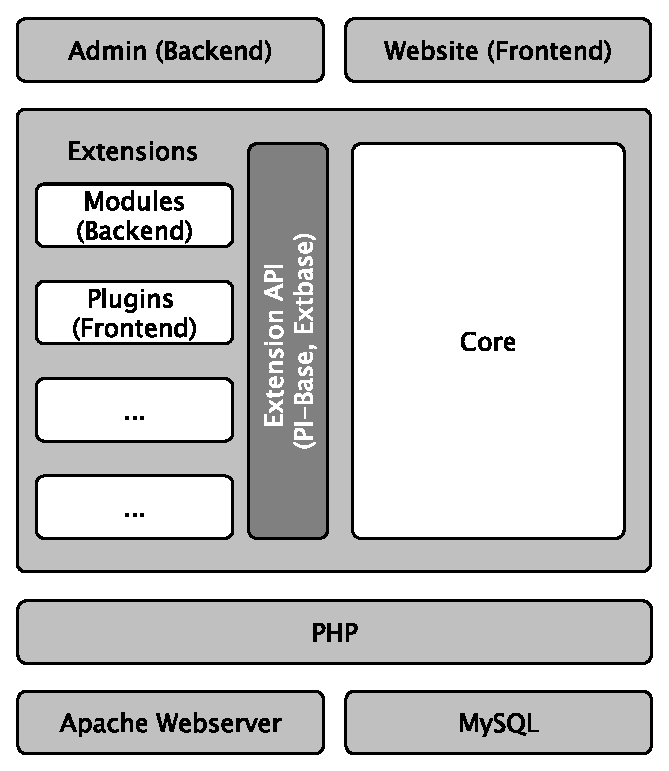
\includegraphics[scale=0.77]{diagrams/TYPO3Architecture.eps}
	\caption{Schematischer Aufbau von TYPO3}
	\label{fig:typo3Architecture}
\end{figure}

Die Gesamtheit aller von TYPO3 CMS zur Verfügung gestellten \gls{api}s, wird als die \mbox{\textit{TYPO3 API}} bezeichnet. Diese kann - analog zum Konzept von Backend und Frontend - in eine \mbox{\textit{Backend \gls{api}}} und eine \mbox{\textit{Frontend \gls{api}}} unterteilt werden. Die Aufgabe der Frontend \gls{api} ist die Zusammenführung der getrennt vorliegenden Bestandteile (Inhalt, Struktur und Layout) aus der Datenbank oder dem Cache zu einer HTML-Seite. Die Backend \gls{api} stellt Funktionen zur Erstellung und Bearbeitung von Inhalten zur Verfügung. (vgl. \cite[S. 5 ff.]{book:dulepovTypo32008})

Die \gls{api}s, die keiner der beiden Kategorien zugeordnet werden kann, bezeichnet Dulepov \cite[S. 5 ff.]{book:dulepovTypo32008} als \mbox{\textit{Common-\gls{api}}}. Die Funktionen der Common-\gls{api} werden von allen anderen \gls{api}s genutzt. Ein Beispiel dafür stellt die Datenbank \gls{api} dar, welche in der Regel nur einfache Funktionen wie das Erstellen, Einfügen, Aktualisieren, Löschen und Leeren\footnote{CRUD - {\bfseries C}reate, {\bfseries R}etrieve, {\bfseries U}pdate und {\bfseries D}elete \label{ft:crud}} von Datensätzen bereitzustellen hat. Auf die aktuelle Datenbank-\gls{api} wird in Kapitel \ref{sec:currentSituation} näher eingegangen.

\subsubsection{XCLASS}
TYPO3 CMS besitzt einen – als XCLASS bezeichneten – Mechanismus, der es erlaubt Klassen zu erweitern oder Methoden mit eigenem Code zu überschreiben. Dies funktioniert für den Systemkern wie auch für andere Extensions. Damit eine Klasse per XCLASS erweiterbar ist, darf sie nicht per \phpinline{new()} Operator erzeugt werden, sondern durch \phpinline{\TYPO3\CMS\Core\Utility\GeneralUtility::makeInstance()}.
Diese Methode sucht im globalen \gls{php}-Array \phpinline{$GLOBALS['TYPO3_CONF_VARS']['SYS']['Objects']} nach angemeldeten Klassen, instanziiert diese und liefert sie anstelle der Originalklasse zurück. Dieses Array dient der Verwaltung der zu überschreibenden Klassen und erfolgt in der Datei \pdf{ext\_localconf.php} innerhalb des Extensionsverzeichnisses.

Der Mechanismus hat jedoch ein paar Einschränkungen:

\begin{itemize}
	\itemsep1pt\parskip0pt\parsep0pt
	\item
		der Code der Originalklasse kann sich ändern. Es ist somit nicht sichergestellt, dass der überschreibende Code weiterhin das macht, wofür er gedacht war
	\item
		XCLASSes funktionieren nicht mit statischen Klassen, statischen Methoden und finalen Klassen
	\item
		eine Originalklasse kann nur einmal per XCLASS überschrieben werden
	\item
		einige Klassen werden sehr früh bei der Initialisierung des Systems instanziiert. Das kann dazu führen, dass Klassen die als Singleton ausgeführt sind, nicht überschrieben werden können oder es kann zu unvorhergesehenen Nebeneffekten kommen.
\end{itemize}

\subsection{Extensions}
Extensions sind funktionale Erweiterungen, die in System-, globale und lokale Extensions unterteilt werden. Sie interagieren mit dem Systemkern über die Extension API und stellen die Möglichkeit dar TYPO3 CMS zu erweitern und anzupassen.

Systemextensions werden mit dem System mitgeliefert und befinden sich ausschließlich im Ordner \pdf{typo3/sysext/}. Sie werden nochmals unterteilt in jene, die für den Betrieb von TYPO3 CMS unabdingbar sind und solche die nicht zwangsläufig installiert sein müssen, jedoch wichtige Funktionen beisteuern.

Neben Systemextensions gibt es globale\footnote{Da globale Extensions nur in bestimmten Szenarien einen Sinn ergeben und in der Realität so gut wie nicht vorkommen, wird von der TYPO3 Community der Begriff "Extension" synonym zum Begriff "lokale Extension" verwendet. Die Arbeit folgt dieser Regelung.} und lokale Extensions. Lokale Extensions werden im Ordner \pdf{typo3conf/ext/} und globale Extensions im Ordner \pdf{typo3/ext} installiert.

\subsubsection{Extension Manager}
Der \gls{em} ist ein \gls{be} Modul, über das die Extensions verwaltet werden können. Es erlaubt die Aktivierung, Deaktivierung, das Herunterladen und das Löschen von Extensions. Darüber hinaus bietet der \gls{em} Möglichkeiten zur detaillierten Anzeige von Informationen über die Extensions wie das Changelog, Angaben zu den Autoren und Ansicht der Dateien der Extension.

